\section{Group Actions}
It is often easier to understand a group if it's doing something, permuting elements, rotating a square etc.

\begin{definition}[Group action]
    Let $G$ be a group and $X$ a non-empty set.
    We say that $G$ \emph{acts} on $X$ if there is a mapping
    \begin{align*}
        \rho : G \times X &\to X \\
        (g, x) &\mapsto \rho(g, x) = g(x)
    \end{align*} 
    such that 
    \begin{enumerate} \addtocounter{enumi}{-1}
        \item if $g \in G$, $x \in X$, then $\rho(g, x) = g(x) \in X$ (implied by notation, but something we should check).
        \item $\rho(gh, x) = \rho(g, \rho(h, x))$. shorthand: $gh(x) = g(h(x))$. \label{action-1}
        \item $\rho(e, x) = x$, shorthand: $e(x) = x$.
    \end{enumerate} 
    When $G$ acts on a set it maps elements of $X$ to $X$ in a way that the multiplication of $G$ is respected.
\end{definition} 

\begin{example}
    \begin{enumerate} \def\labelenumi{\roman{enumi}.} \def\labelenumii{\arabic{enumii}.} 
        \item trivial action $\rho(g, x) = x \; \forall \; x_in X, g \in G$.
        \item $S_n$ acts on $X = \{ 1, 2, \ldots, n \}$ by permuting the elements of $X$.
        e.g. $S_3$ acts on $\{1, 2, 3\}$, $\sigma = \begin{pmatrix}1 & 2\end{pmatrix} \in S_3 : \sigma(1) = 2, \sigma(2) = 1, \sigma(3) = 3$.
        $\tau = \begin{pmatrix}1 & 3\end{pmatrix} \in S_3$, $\tau \sigma = \begin{pmatrix}1 & 3\end{pmatrix} \begin{pmatrix}1 & 2\end{pmatrix} = \begin{pmatrix}1 & 2 & 3\end{pmatrix}$ \\
        $(\tau \sigma)(1) = 2$, $\tau(\sigma(1)) = \tau(2) = 3$. \\
        Similarly subgroups of $S_n$ act on $X$.
        \item $D_8 = \{e, r, r^2, r^3, t, rt, r^2t, r^3t \}$ acts on the edges of a square.
        \begin{figure}
            \centering 
            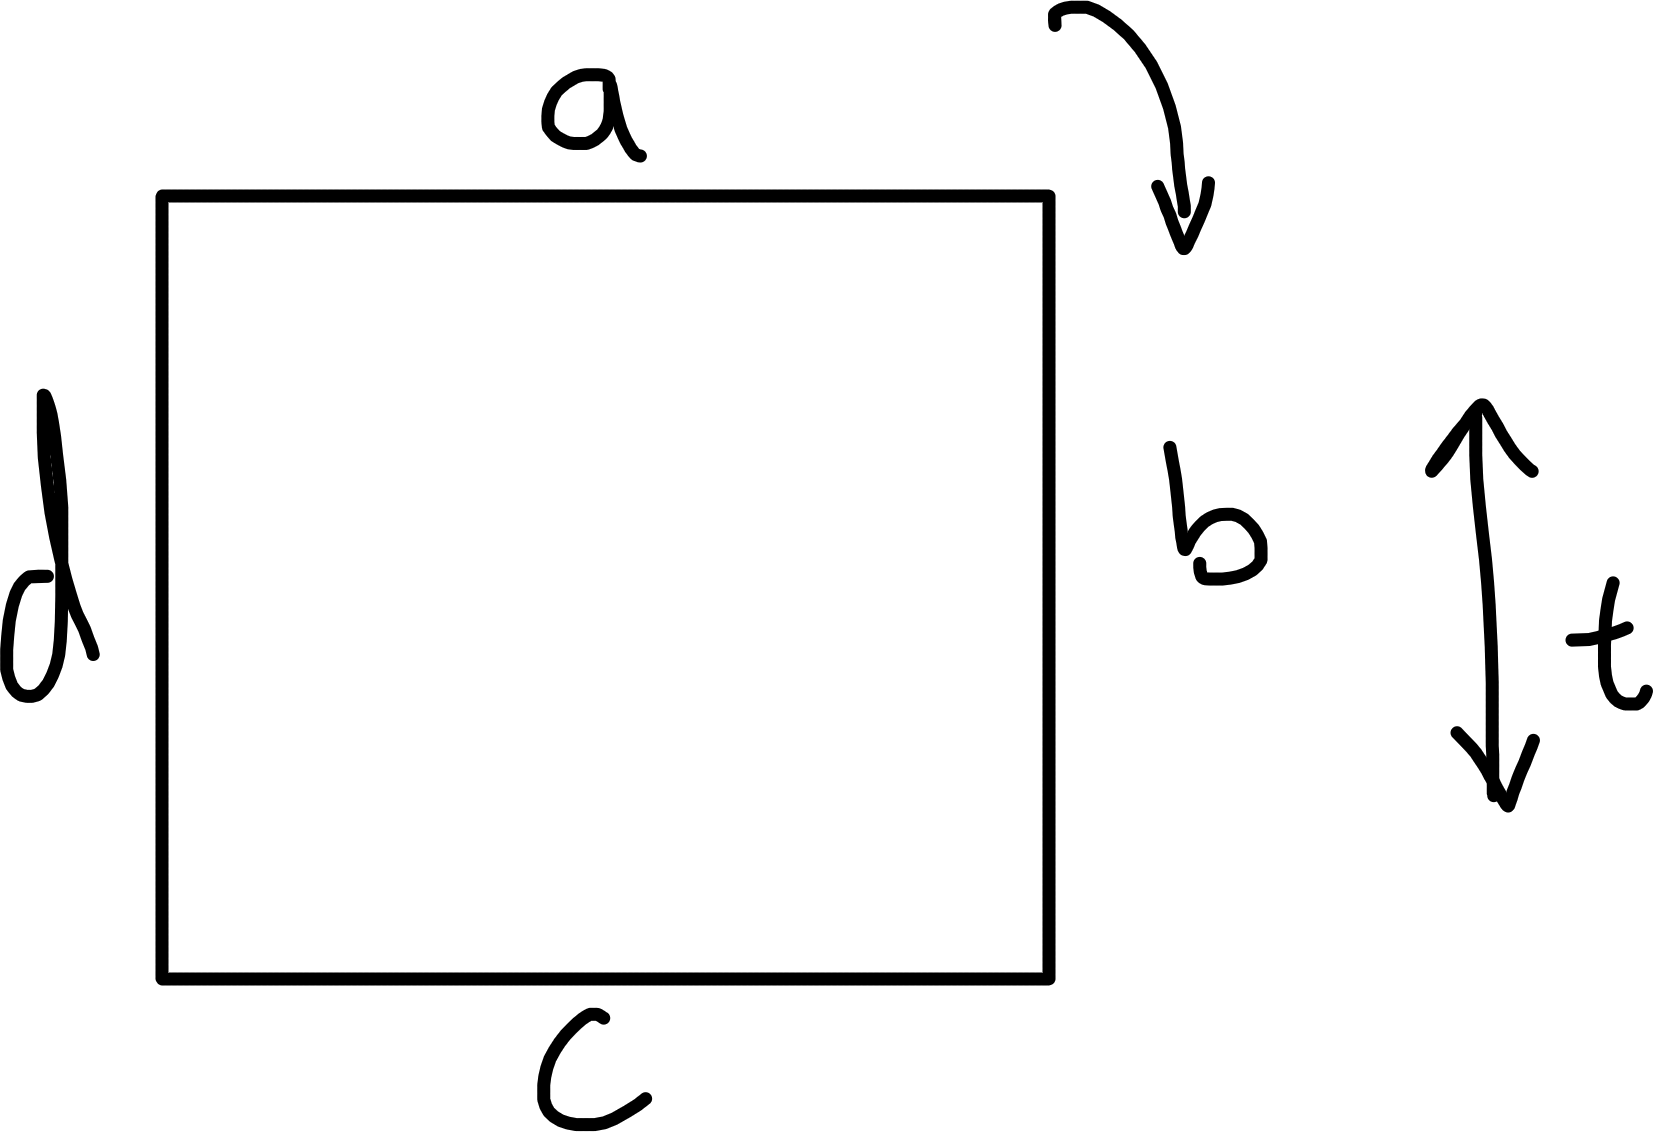
\includegraphics[height=5cm]{figures/06-square-action}
        \end{figure} 
        \begin{align*}
            t(a) &= c & t(c) &= a \\
            t(b) &= b & t(d) &= d. \\
            s(a) &= b. (r?)
        \end{align*} 
        Also acts on the vertices of a square.
        \begin{figure}
            \centering 
            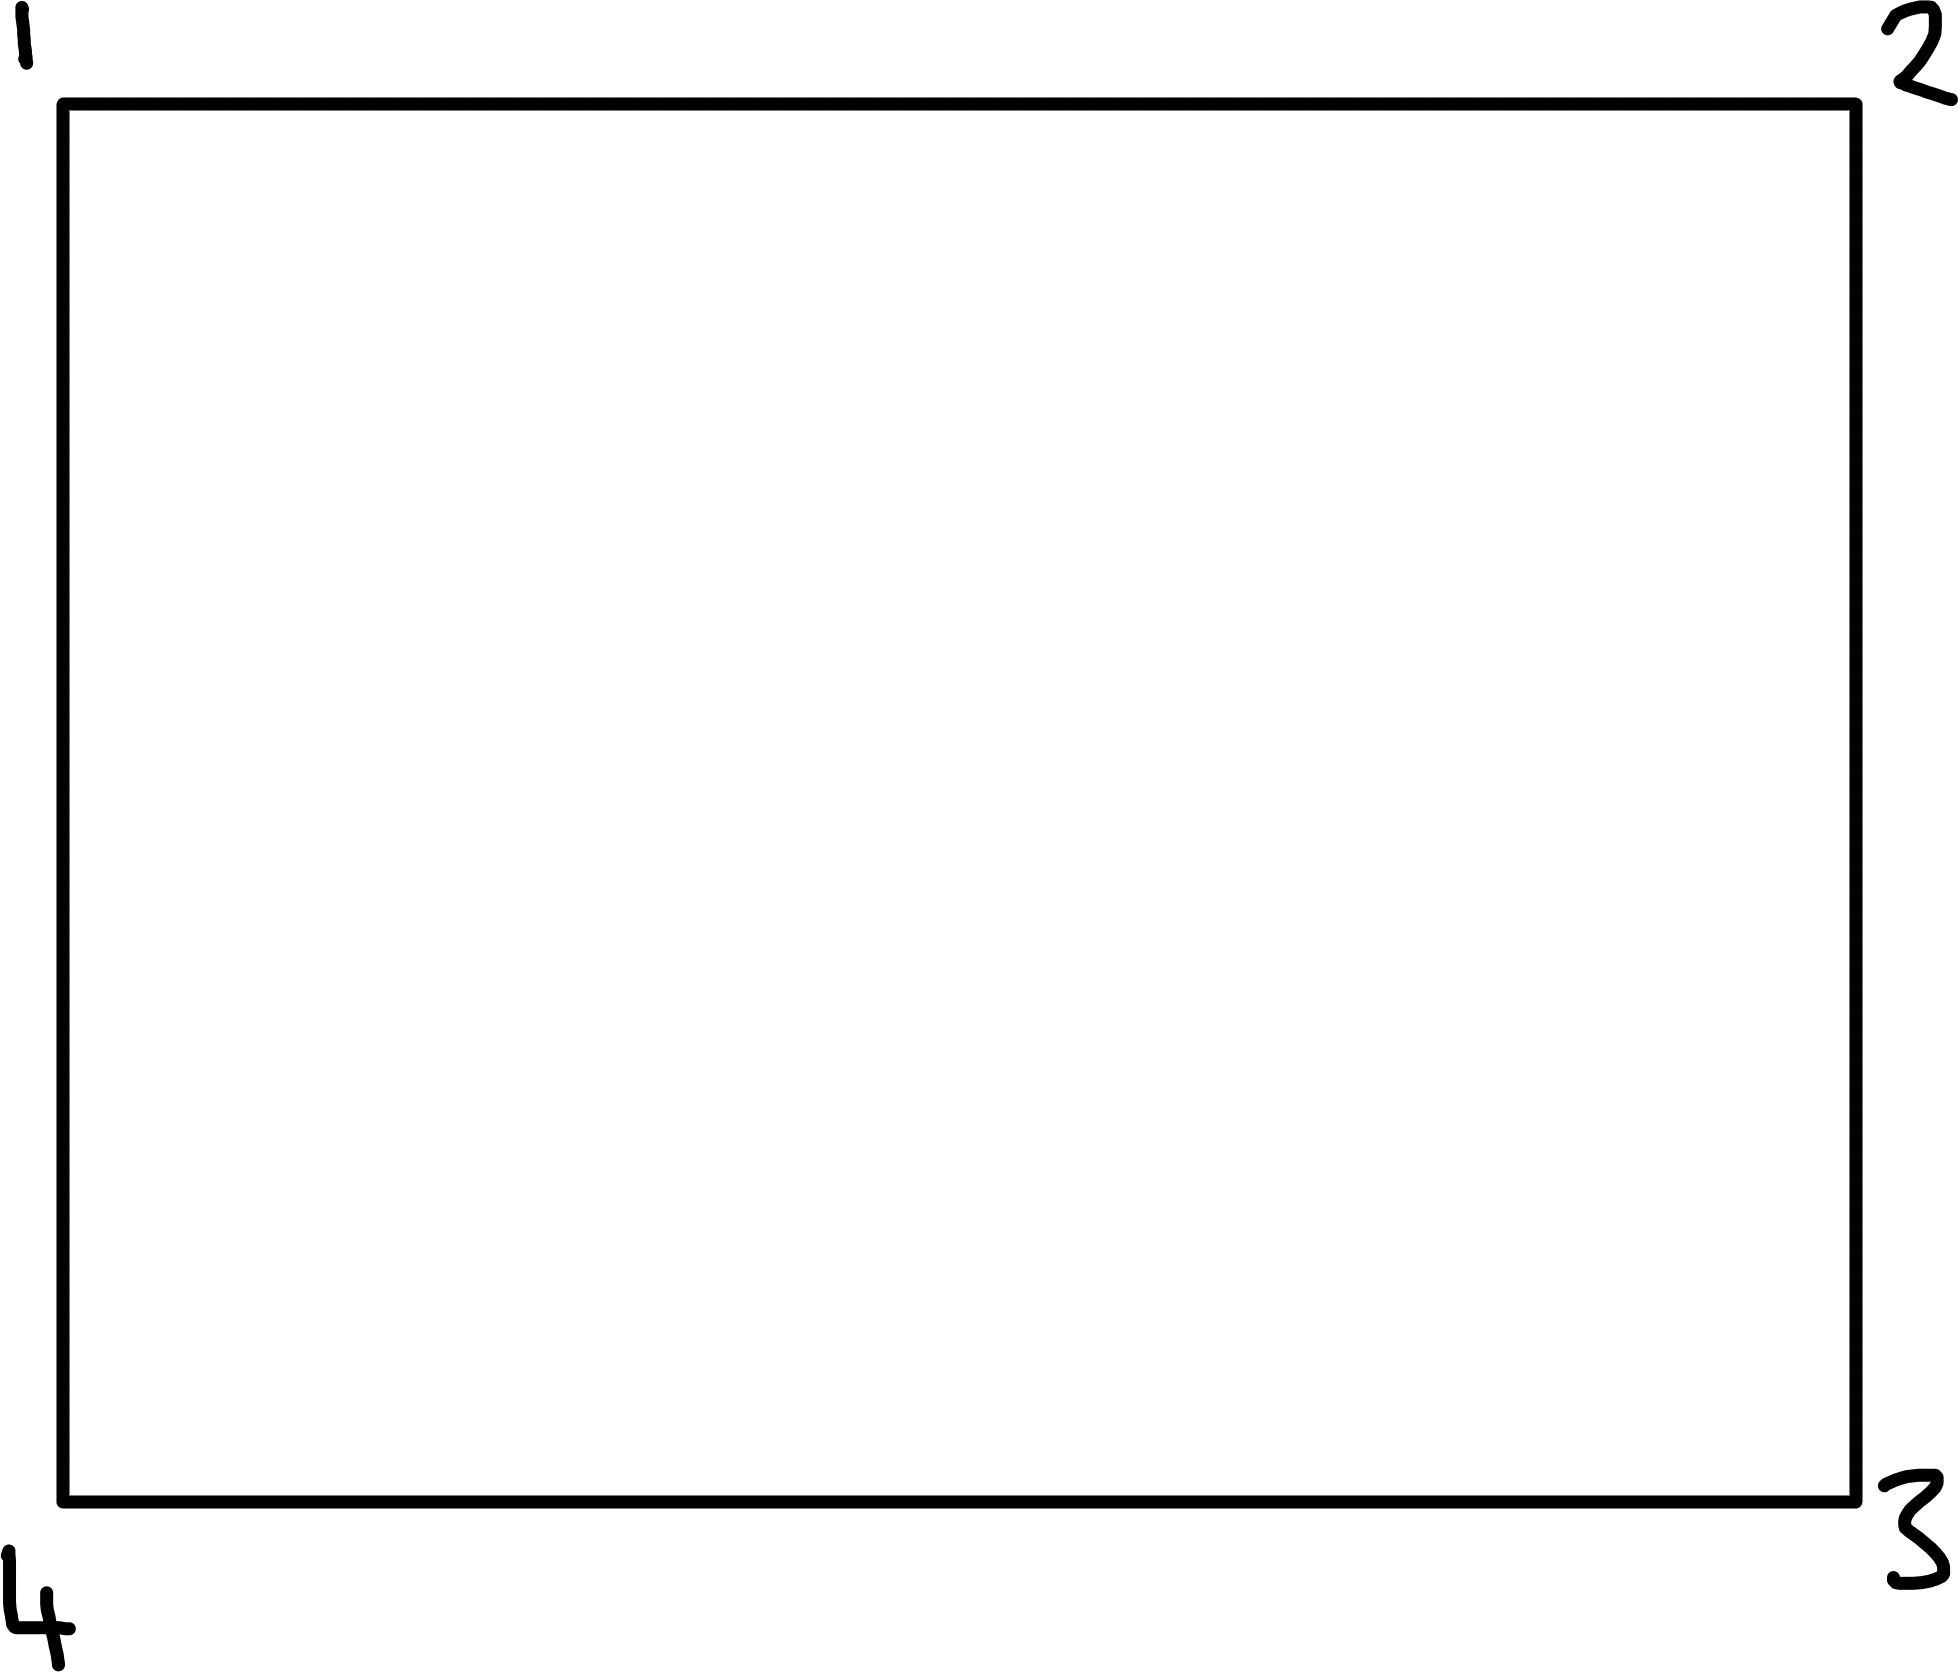
\includegraphics[height=5cm]{figures/06-square-action-vertex}
        \end{figure} 
        \begin{align*}
            t(1) &= 4 & t(4) &= 1 \\
            t(2) &= 3 & t(d) &= 2. \\
        \end{align*} 
        \item $G$ acts on itself by left multiplication.
        This is called the \emph{left regular action}
        \begin{align*}
            G \times G &\to G \\
            (g, k) &\mapsto gk.
        \end{align*} 
        Check:
        \begin{enumerate} \addtocounter{enumii}{-1}
            \item $gk \in G$ (by closure)
            \item
            \begin{align*}
                \rho(gh, k) &= ghk \\
                \rho(g, \rho(h, k)) &= \rho(g, hk) = ghk \\
                \intertext{Or in shorthand: }
                gh(k) &= ghk \\
                g(h(k)) &= g(hk) = ghk.
            \end{align*} 
            \item $\rho(e, k) = ek = k$.
        \end{enumerate} 
        \item We also have the $G$ \emph{right regular action}
        \begin{align*}
            G \times G &\to G \\
            (g, k) &\mapsto k g^{-1}.
        \end{align*} (we need inverse for \Cref{action-1} to hold.)
        \item $G$ acts on itself by \emph{conjugation}
        \begin{align*}
            G \times G &\to G \\
            (g, k) &\mapsto gkg^{-1}.
        \end{align*} 
        Check: 
        \begin{enumerate} \addtocounter{enumii}{-1}
            \item $gkg^{-1} \in G$ (by closure)
            \item
            \begin{align*}
                \rho(gh, k) &= ghk(gh)^{-1} \\
                &= gh k h^{-1} g^{-1}
                \rho(g, \rho(h, k)) &= \rho(g, hkh^{-1}) = g (h k h^{-1}) g^{-1} \\
            \end{align*} 
            \item $\rho(e, k) = ek e^{-1} = k$.
        \end{enumerate} 
        \item Let $N \trianglelefteq G$, then $G$ acts on $N$ by conjugation
        \begin{align*}
            G \times N &\to N \\
            (g, n) &\mapsto gng^{-1}.
        \end{align*} 
        0.  $gng^{-1} \in G$ since $N \trianglelefteq G$
        (1) and (2) as above.
        \item Let $H \leq G$, then $G$ acts on the set of left cosets, $(G : H)$, if $H$ in $G$.
        Called the \emph{left coset action}.
        \begin{align*}
            G \times (G : H) &\to (G : H) \\
            (g, kH) &\mapsto gkH.
        \end{align*} 
        \begin{enumerate} \addtocounter{enumii}{-1}
            \item $gkH \in (G : H)$
            \item
            \begin{align*}
                \rho(gh, kH) &= (gh)kH = gh kH. \\
                \rho(g, \rho(h, kH)) &= \rho(g, hkH) \\
                &= g h k H \\
            \end{align*} 
            \item $\rho(e, kH) = ek H = kH$.
        \end{enumerate} 
    \end{enumerate} 
\end{example} 

\begin{remark}
    Recall a permutation of a set $X$ is a bijection of $X$, \Cref{def:permutation}.
    We have commented that a bijection $f : X \to X$ has a 2-sided inverse, i.e. $\exists \; g : X \to X$ s.t.
    \begin{align*}
        f \circ g (x) &= x \; \forall \; x \in X \\
        g \circ f (x) &= x \; \forall \; x \in X.
    \end{align*}
    Conversely if $f : X \to X$ is a map with a 2-sided inverse then $f$ is a bijection.
    \begin{align*}
        f \circ g(x) &= x \; \forall \; x \in X \implies f \text{ is surjective, as $f$ is mapping to all elements in $X$} \\
        g \circ f (x) &= x \; \forall \; x \in X \implies f \text{ is injective, as if $f$ took two elements to the same place then $g$ wouldn't be able to split them up}.
    \end{align*} 
    Note 2-sided is necessary:
\end{remark} 